\documentclass[12pt, a4paper]{article}

\usepackage[a4paper, margin=2cm]{geometry}
\usepackage{setspace}
\usepackage[portuguese]{babel}
\usepackage{graphicx}
\usepackage{hyperref}

\chardef\_=`_

\title{\textbf{LI3 - Relatório da Fase I - Grupo 12}}
\author{
    Humberto Gomes (A104348) \\
    José Lopes     (A104541) \\
    José Matos     (A100612) \\
}
\date{novembro de 2023}

\begin{document}
\maketitle
\onehalfspacing
\setlength{\parskip}{\baselineskip}
\setlength{\parindent}{0pt}

\begin{abstract}
    Este relatório tem como intuito explicar a estrutura do nosso trabalho prático para a UC de LI3.
    Como o foco principal desta UC é a modularização e o encapsulamento do código, este documento
    descreve como tal for conseguido, justificando as nossas decisões a este nível. O objetivo do
    projeto para a 1.ª fase é o \emph{parsing} e validação de um \emph{dataset} contendo
    utilizadores, voos, passageiros em voos e reservas de hotéis, sobre o qual serão executadas
    \emph{queries}, das quais implementámos seis, fornecendo informação sobre a base de dados. O
    modo de organização e processamento destes dados também é descrito.
\end{abstract}

\section{Estrutura do trabalho}

Devido ao elevado número de módulos, um diagrama completo de módulos com relações de dependência
não cabe numa página A4, pelo que optámos por fazer vários diagramas, um para cada secção lógica
do programa. Mesmo assim, para reduzir a complexidade visual, não incluímos todas as relações de
dependência, mas apenas as mais relevantes.

A nossa convenção gráfica é a seguinte:

\begin{itemize}
    \item Um retângulo representa um módulo;
    \item Um retângulo com cantos arredondados representa uma estrutura de dados;
    \item $A \rightarrow B$ significa que o módulo $A$ depende do módulo $B$.
\end{itemize}

\subsection{Subsistema de \emph{Parsing}}
\label{sec:parsing}

\begin{center}
    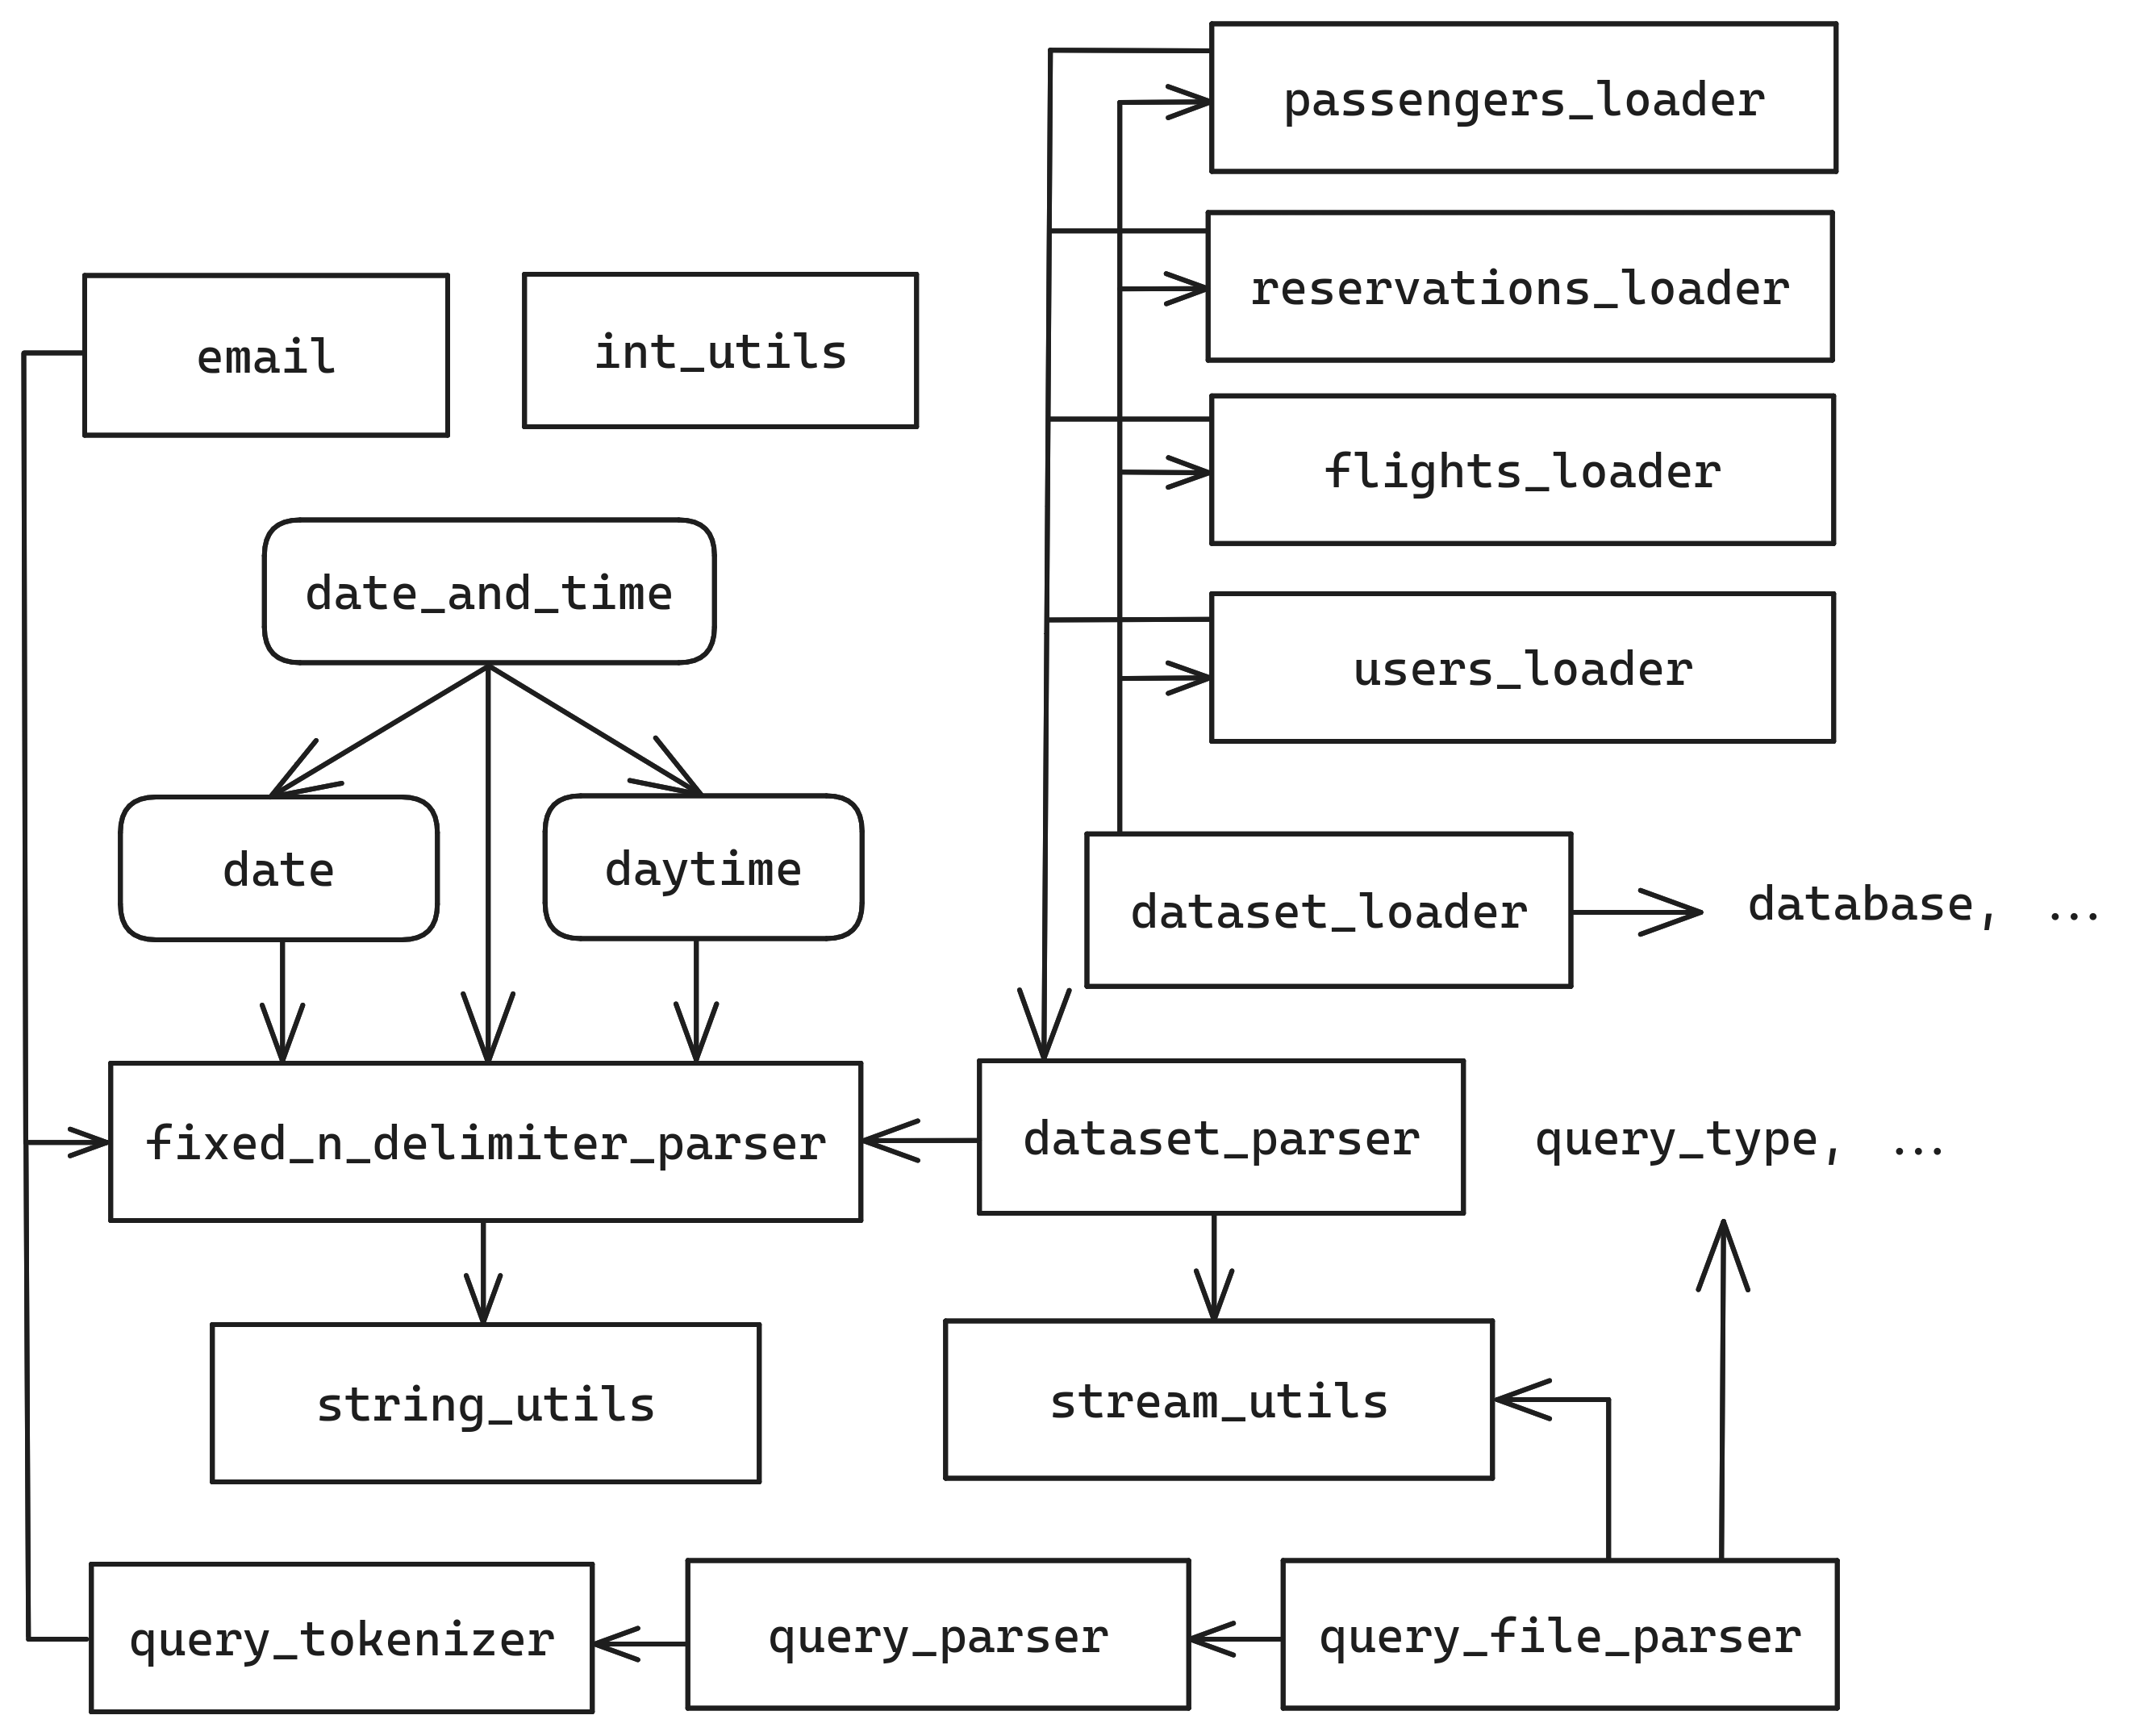
\includegraphics[scale=0.17]{res/parsing.png}
\end{center}

O nosso sistema de \emph{parsing} começa com \emph{tokenizadores}, que separam \emph{strings} e
ficheiros por um delimitador (\texttt{string\_utils} e \texttt{stream\_utils}, respetivamente).
Sobre estes é construído o caso mais específico do \texttt{fixed\_n\_delimiter\_parser}, que espera
um número pré-determinado de \emph{tokens}, chamando um \emph{callback} diferente para cada um (uma
gramática genérica, definível pelo programador, define estes \emph{callbacks}). Este \emph{parser}
é utilizado para o \emph{parsing} de datas (\texttt{date}), horas de um dia (\texttt{daytime}),
combinações de datas e horas (\texttt{date\_and\_time}), linhas de um \emph{dataset} e validação de
\emph{emails} (\texttt{email}).

Para a análise de um ficheiro de \emph{dataset}, o \texttt{dataset\_parser}, também programável com
uma gramática, é responsável por separar o ficheiro por linhas, excluir a primeira linha de cada
ficheiro (o \emph{header} da tabela CSV), e \emph{tokenizar} cada linha, chamando os
\emph{callbacks} adequados. O \texttt{dataset\_loader}, não propriamente encaixado neste secção de
\emph{parsing}, é responsável por abrir cada ficheiro do \emph{dataset}, interagir com os
\emph{parsers} adequados, adicionando elementos à base de dados e registando os erros por eles
reportados nos ficheiros \texttt{*\_errors.csv}.

O \emph{parsing} de \emph{queries} requer um \emph{tokenizador} separado para lidar com aspas
(\texttt{query\_tokenizer}), um \emph{parser} para determinar o tipo de \emph{query} e se os seus
argumentos são válidos (\texttt{query\_parser}), e um \emph{parser} de um ficheiro com várias
\emph{queries} em várias linhas (\texttt{query\_file\_parser}).

\subsection{Entidades}

\begin{center}
    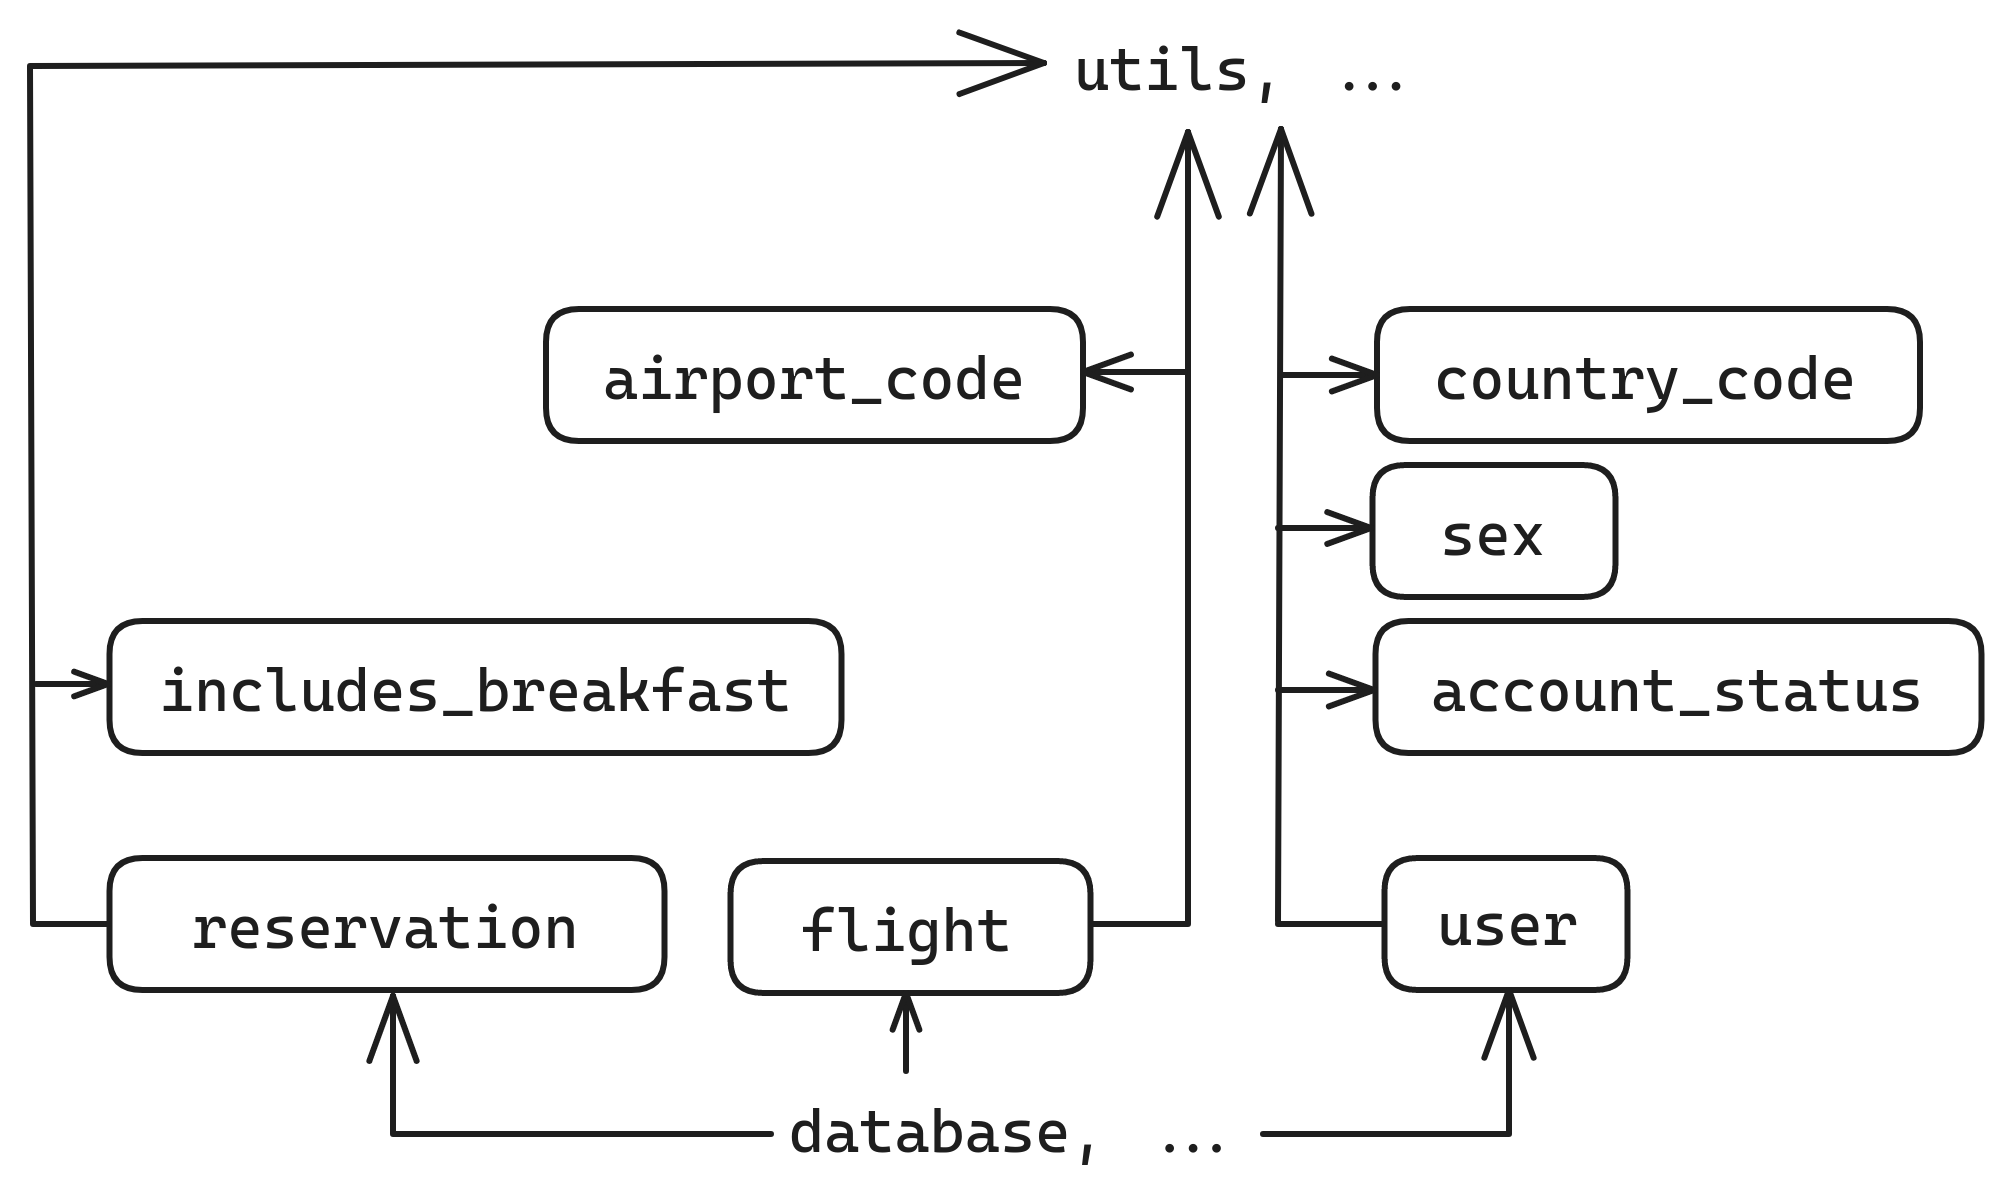
\includegraphics[scale=0.2]{res/entities.png}
\end{center}

O nosso projeto define três entidades (\texttt{user\_t}, \texttt{reservation\_t} e
\texttt{flight\_t}), correspondentes às definidas no enunciado do trabalho, juntamente com módulos
de estruturas de dados auxiliares. Os campos destas entidades formam um subconjunto dos campos
definidos no enunciado do trabalho (não armazenamos campos nunca pedidos por \emph{queries}). A
única exceção ocorre nos voos, onde adicionamos um campo relativo ao número de passageiros, devido
à sua grande utilidade tanto para a validação do \emph{dataset} como para a execução de
\emph{queries}.

\subsection{Catálogos}

\begin{center}
    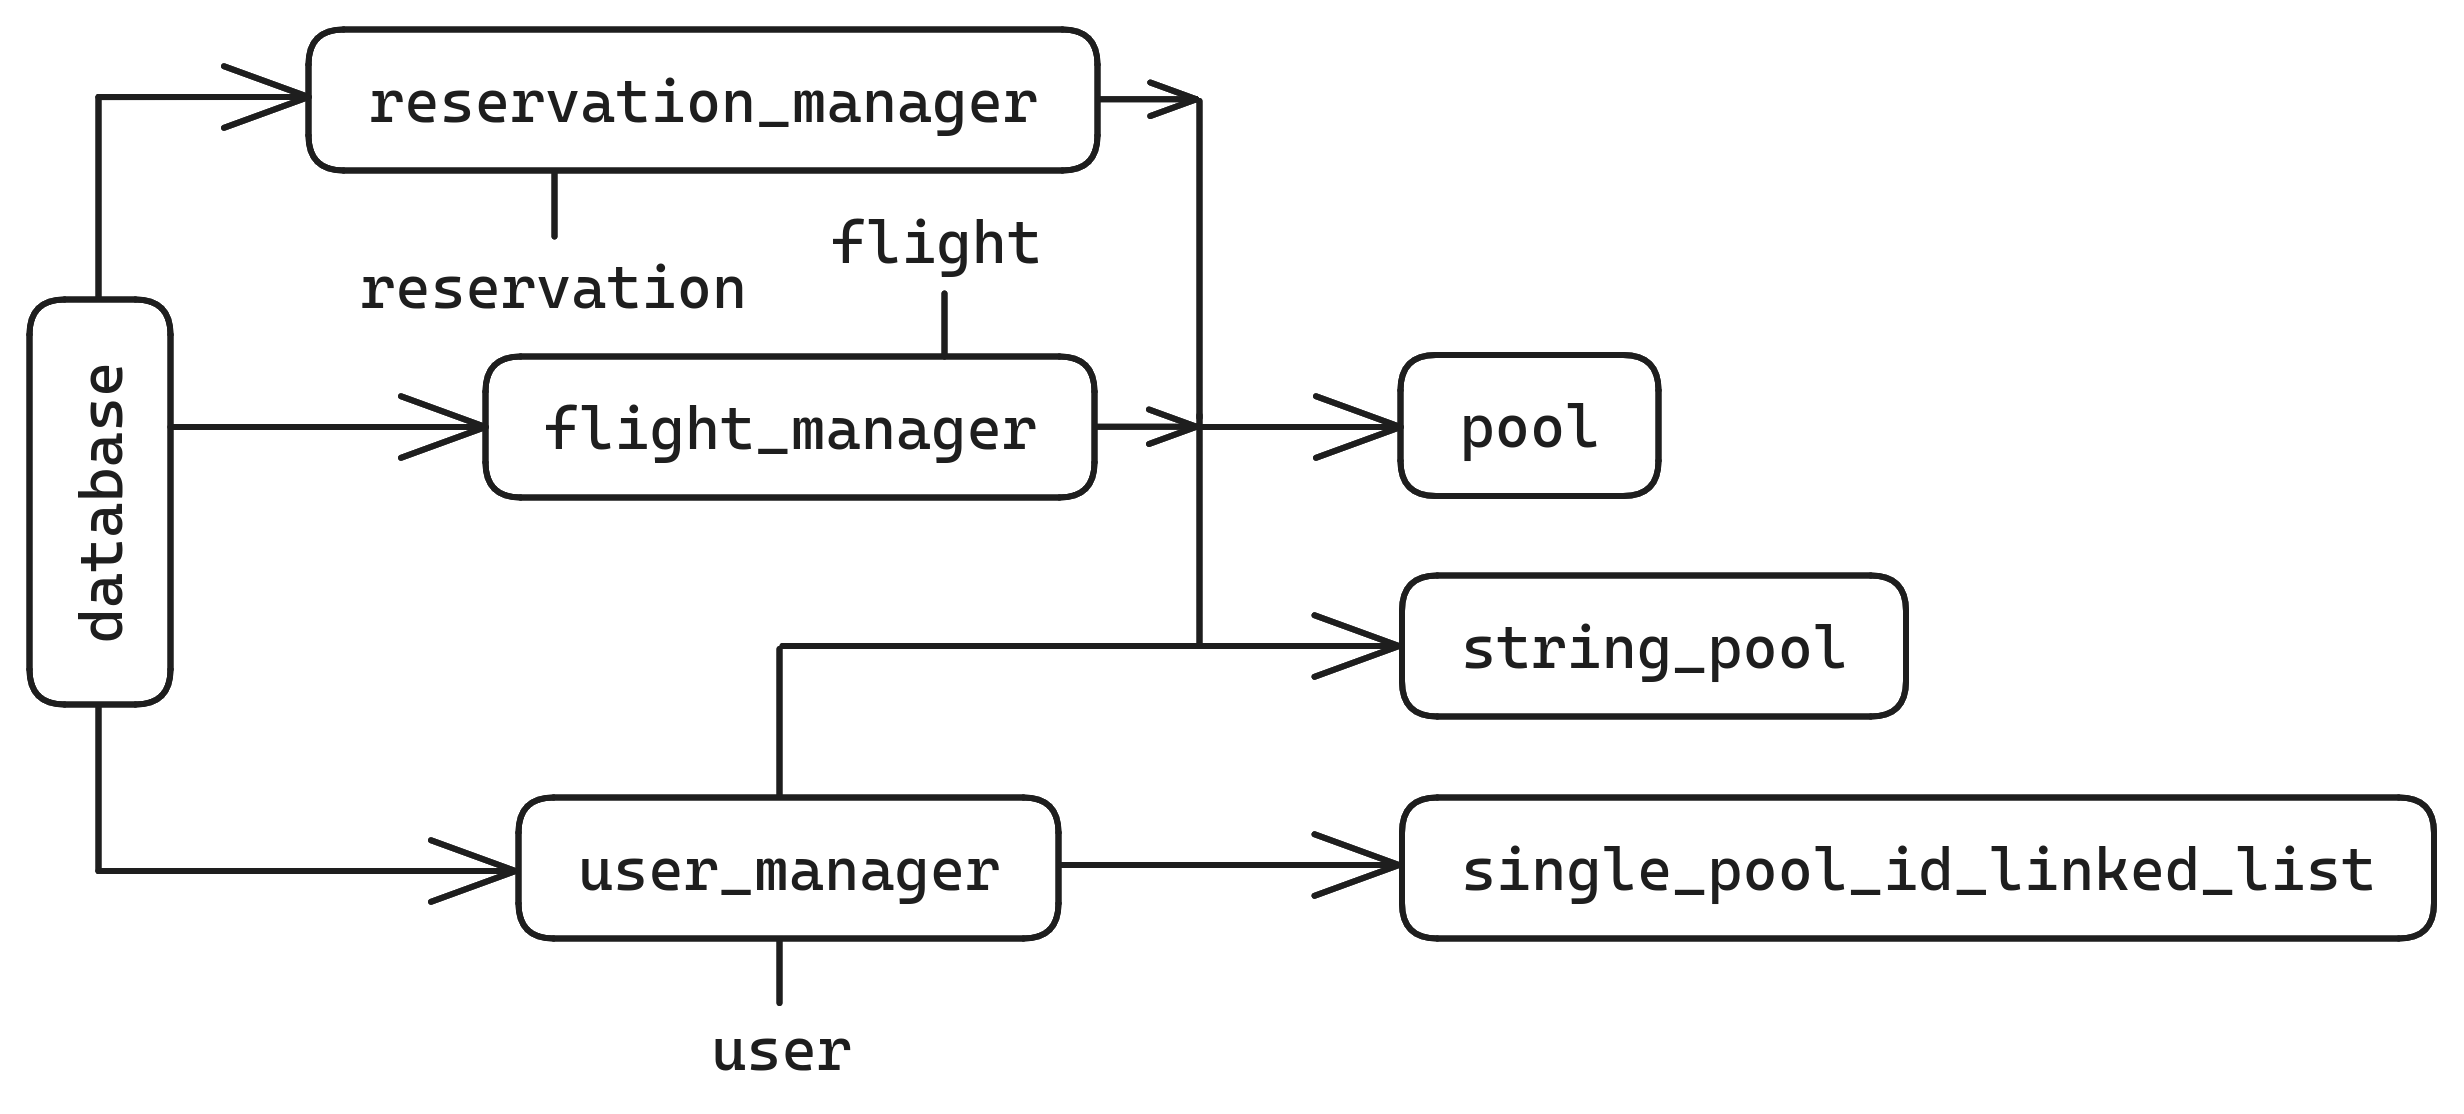
\includegraphics[scale=0.19]{res/database.png}
\end{center}

Antes de definirmos uma base de dados, começámos por definir estruturas que permitem melhorar a
eficiência espacial e a velocidade das alocações na aplicação: um alocador em \texttt{pool} para
objetos todos do mesmo tamanho, e uma \texttt{string\_pool} para \emph{strings}. Uma
\texttt{single\_pool\_id\_linked\_list} é uma implementação de uma lista ligada na qual que várias
listas podem partilhar a mesma \texttt{pool} para armazenamento de nodos, contribuindo para um
menor uso de memória em \emph{overheads} de alocação.

No módulo \texttt{database}, definimos uma estrutura de dados que contém os três \emph{managers} na
aplicação: o \texttt{reservation\_manager}, que gere reservas, o \texttt{flight\_manager}, que gere
voos, e o \texttt{user\_manager}, que gere utilizadores, ligando também cada utilizador aos
identificadores de voos e reservas a ele associados. Todos estes \emph{managers} consistem numa
\texttt{pool} para alocação de entidades, uma \texttt{string\_pool} para alocação de \emph{strings},
e uma tabela de \emph{hash}, para a associação de identificadores de entidades às entidades em si.
O \texttt{user\_manager} surge como exceção, onde cada identificador de um \texttt{user} se
encontra também associado a listas ligadas com os IDs dos voos e reservas associados a esse
utilizador.

\subsection{\emph{Queries}}

\begin{center}
    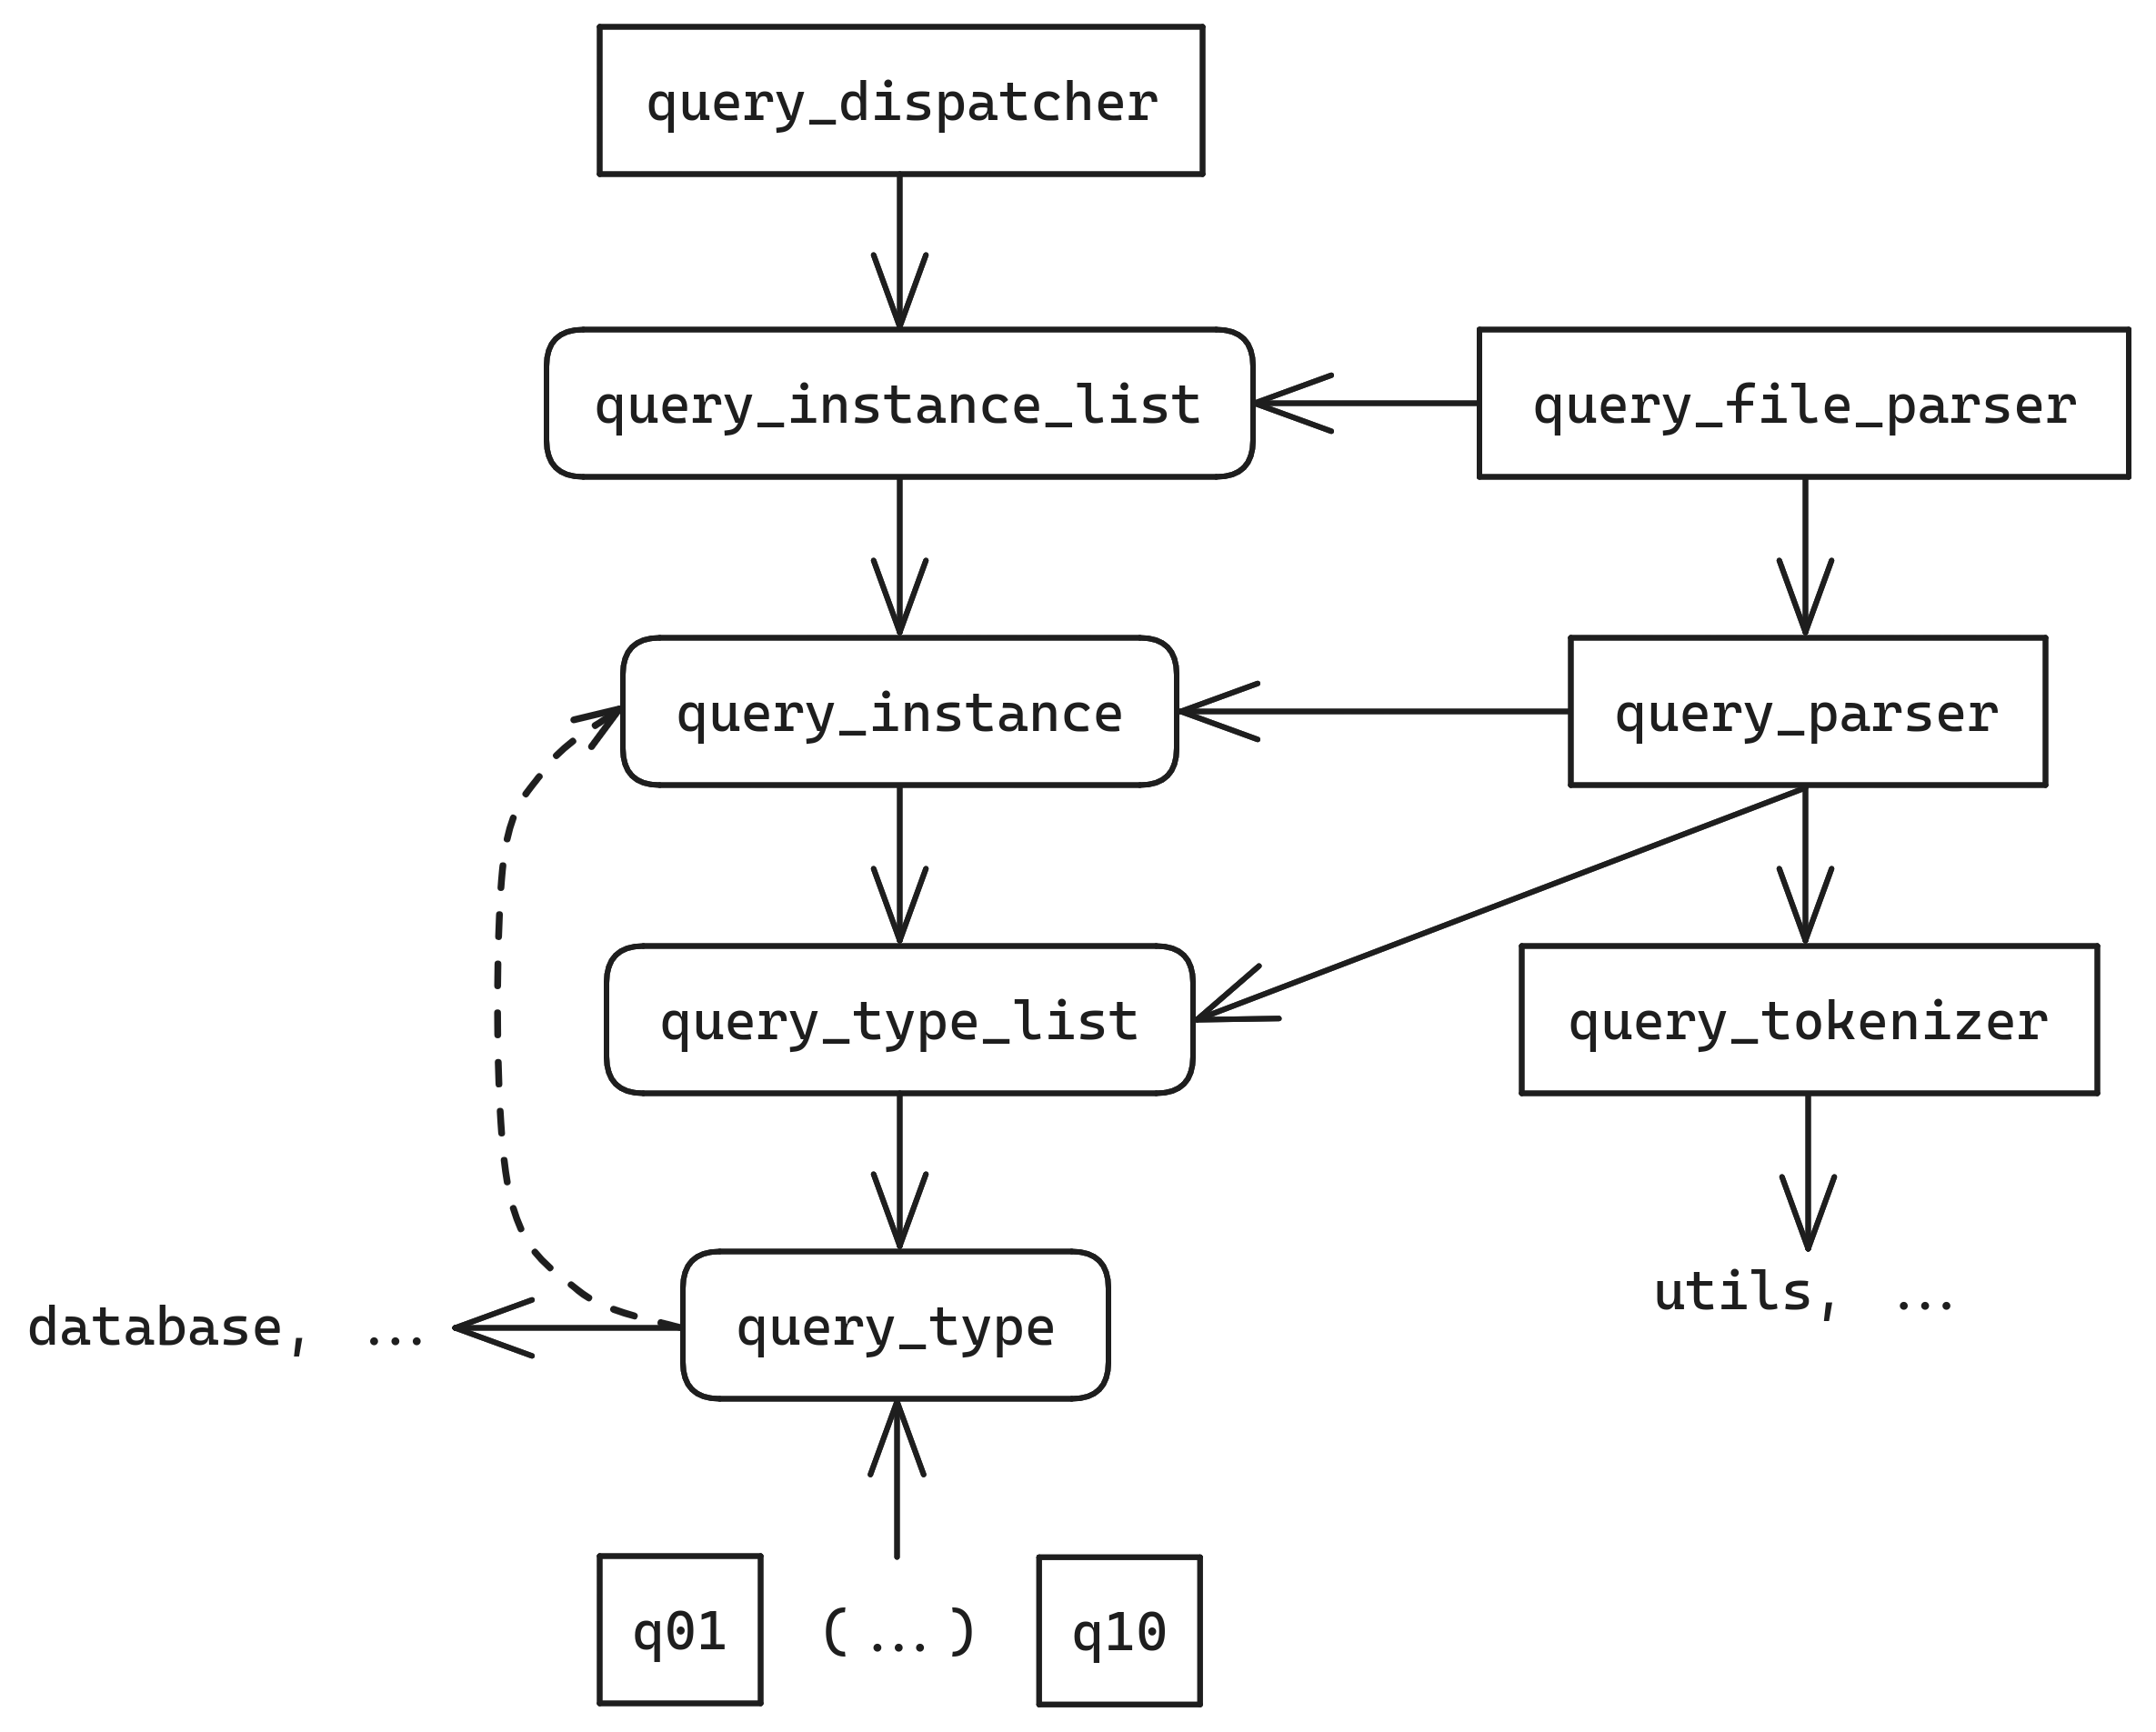
\includegraphics[scale=0.19]{res/queries.png}
\end{center}

O \emph{parsing} de \emph{queries} já foi descrito na secção \nameref{sec:parsing}. No sistema de
\emph{queries}, começámos por definir um \texttt{query\_type}, um conjunto de \emph{callbacks} que
define uma \emph{query}, de modo a se simular polimorfismo em C. Definir uma \emph{query} resume-se
a a definir uma função para cada \emph{callback}, e adicioná-la à \texttt{query\_type\_list}, a
lista de todas as \emph{queries} conhecidas.

Antes de enumerar as \emph{queries} implementadas, devemos mencionar como geramos dados estatísticos
para uma \emph{query}. Ao contrário do sugerido no enunciado no projeto, não utilizamos um módulo
para estatísticas, dado que implementá-lo seria uma quebra do modularidade da aplicação: implementar
uma nova \emph{query} implicaria edições consideráveis a vários módulos. Sendo assim, optámos por um
modelo em que dados estatísticos são gerados por cada tipo (número) de \emph{query}, e são
partilhados por todas as \emph{queries} do mesmo tipo. Por exemplo, torna-se possível fazer uma
única iteração da base de dados para todas as \emph{queries} do tipo 3, em vez de uma iteração para
cada \emph{query} deste tipo. Assim, temos uma solução mais modular, mas com pior desempenho do que
um módulo de estatísticas globais (que faria uma única iteração pelos dados).

Estas são as \emph{queries} que implementámos nesta primeira fase:

\begin{itemize}
    \item \textbf{Q01} - Consulta de uma entidade pelo seu identificador. A sua implementação foi
                         trivial: começa-se por determinar o tipo da entidade com base no formato
                         do seu identificador, processo seguido da consulta direta do \emph{manager}
                         correto na base de dados.

    \item \textbf{Q02} - Listagem de voos e / ou reservas de um utilizador. Também de implementação
                         trivial, esta \emph{query} pede a lista de reservas / voos (ou ambas) de um
                         utilizador ao \texttt{user\_manager} (consulta direta), seguida da consulta
                         também direta do \emph{manager} adequado para cada voo / reserva, para a
                         obtenção de informação sobre data do evento.

    \item \textbf{Q03} - Apresentação da classificação média de um hotel. Numa única iteração
                         estatística pelas reservas, calcula-se a média de todos os hotéis
                         mencionados nas \emph{queries} de tipo 3. A execução de cada \emph{query}
                         resume-se então à consulta direta dos dados estatísticos, formados por uma
                         tabela de \emph{hash} que associa o identificador de um hotel à sua média.

    \item \textbf{Q04} - Listagem das reservas de um hotel. Tal como a Q03, faz-se uma única
                         iteração estatística da lista de reservas, mas em vez de se calcular uma
                         média com cada reserva, adiciona-se a reserva a um \emph{array} associado
                         a esse hotel através de uma tabela de \emph{hash}. Após se ordenar cada
                         \emph{array}, pode-se proceder à execução de cada \emph{query}, uma
                         consulta direta dos dados estatísticos.

    \item \textbf{Q06} - Listagem dos $N$ aeroportos com mais passageiros num dado ano. Com uma
                         única iteração estatística pelo \texttt{flight\_manager}, forma-se uma
                         tabela de \emph{hash}, que associa anos a outras tabelas de \emph{hash},
                         que por sua vez associam aeroportos a números de passageiros. Cada uma
                         destas segundas tabelas de \emph{hash} é convertida para um \emph{array}
                         ordenado de pares aeroporto-passageiros. Assim, a execução de uma
                         \emph{query} limita-se à escolha do \emph{array} de pares corretos e à
                         apresentação dos seus primeiros $N$ elementos.

    \item \textbf{Q09} - Listagem de todos os utilizadores cujo nome tenha como prefixo o argumento
                         desta \emph{query}. De momento, devido ao breve prazo de entrega,
                         implementámos esta \emph{query} ineficientemente, com uma iteração do
                         gestor de utilizadores e filtragem dos nomes por cada \emph{query} no
                         ficheiro de \emph{input}. Segue-se a ordernação e apresentação dos
                         resultados. Pretendemos melhorar esta \emph{query} na segunda fase,
                         adicionando uma árvore binária de procura com os nomes dos utilizadores
                         ao \texttt{user\_manager}.
\end{itemize}

Retornando à descrição de cada módulo, uma \texttt{query\_instance} refere-se à ocorrência de uma
\emph{query} (num ficheiro, por exemplo), e uma \texttt{query\_instance\_list} a uma lista destas.
Por último, o \texttt{query\_dispatcher} é o módulo responsável por executar uma lista de
\emph{queries} dada uma base de dados e os ficheiros de \emph{output} de cada \emph{query}.




\section{Otimização do uso de memória}

Dado que os \emph{datasets} da 2.ª fase serão de maior dimensão, preocupámo-nos desde já com a
quantidade de memória utilizada, de modo não sermos futuramente obrigados a reescrever partes
significativas do nosso código.

\subsection{Observação do \emph{dataset} e das \emph{queries}}

Pudemos observar que alguns campos do \emph{dataset} nunca precisavam de estar presentes no
\emph{output} de nenhuma \emph{query} (ex: o \emph{email} de um utilizador), pelo que era escusado
o seu armazenamento na base de dados, sendo apenas necessária a sua validação durante o
\emph{parsing}. Ademais, por observação dos \emph{datasets} em si, pudemos concluir que é possível
armazenar certos campos como estruturas de dados mais compactas (ex: o identificador de um voo
pode ser armazenado como um inteiro, em vez de uma \emph{string}).

\subsection{Tipos opacos}

Um dos nossos obstáculos principais foi a forma como tipos opacos são implementados em C, que,
devido à sua natureza de apontador, exigem uma alocação por cada instanciamento. Esta secção
descreve como, mantendo o encapsulamento dos tipos, conseguimos definir tipos de dados opacos sem
estas limitações.

\subsubsection{Datas e horas}

De modo à \texttt{struct} de uma entidade (como um utilizador) poder conter, no seu interior, uma
data ou uma hora, sem alocações, estas são representadas como inteiros. Para modificar estes
inteiros, o módulo do tipo de dados usa uma \texttt{union}, como é visível abaixo no exemplo das
datas:


\begin{spacing}{1}
\begin{center}
    \begin{tabular}{ |l|l| }
        \hline
        \emph{include/utils/date.h}: & \emph{src/utils/date.c}: \\
        & \\
        \texttt{typedef int32\_t date\_t;} & \texttt{typedef union \{} \\
                                           & \texttt{\hspace{0.5cm}date\_t date;} \\
                                           & \texttt{} \\
                                           & \texttt{\hspace{0.5cm}struct \{} \\
                                           & \texttt{\hspace{1cm}uint16\_t year;} \\
                                           & \texttt{\hspace{1cm}uint8\_t month, day;} \\
                                           & \texttt{\hspace{0.5cm}\} fields;} \\
                                           & \texttt{\} date\_union\_helper\_t;} \\
        \hline
    \end{tabular}
\end{center}
\end{spacing}

\subsubsection{Alocação de entidades em \emph{pools}}

Para evitar uma chamada de \texttt{malloc} por cada entidade no \emph{dataset}, procurámos alocar
grandes blocos contíguos de memória de uma vez (\emph{pools}), cada um contendo várias entidades.
No entanto, como o único aspeto de um tipo opaco exposto no \emph{header file} é um apontador, não
se sabe o tamanho da estrutura inerente a que o apontador se refere, impossibilitando a existência
destas \emph{pools}. Para endereçar este problema, adicionámos um método \texttt{\_sizeof} a cada
entidade que pretendíamos colocar em \emph{pools} (ex: \texttt{user\_sizeof}). A implementação
deste método, no ficheiro C, tem acesso à \texttt{struct} interna, podendo simplesmente ser
implementado como \texttt{return sizeof(user\_t);}.

\end{document}
